\documentclass{beamer}

\mode<presentation>
{
  \usetheme{Hannover}      % or try Darmstadt, Madrid, Warsaw, ...
  \usecolortheme{sidebartab} % or try albatross, beaver, crane, ...
  \usefonttheme{default}  % or try serif, structurebold, ...
  \setbeamertemplate{navigation symbols}{}
  \setbeamertemplate{caption}[numbered]
} 

\usepackage[english]{babel}
\usepackage[utf8x]{inputenc}
\usepackage{tikz}
\usetikzlibrary{shapes,arrows}
\usepackage{empheq}
\usepackage{amsmath,amssymb}
\usepackage{MnSymbol}
\usepackage{bbm,dsfont}

\title[MW Algorithm]{The Multiplicative Weights Update Method:}
\subtitle{Applications to Linear Programming and Semidefinite Programming}
\author[Gao, Gaddy]{Zheming Gao and Missy Gaddy}
\institute{Based on paper by Arora, Hazan, and Kale (2012)}
\date{November 29, 2017}

\begin{document}
%%%%%%%%%%%%%%%%%
\begin{frame}
  \titlepage
\end{frame}
\begin{frame}{Outline}
  \tableofcontents 
\end{frame}

%%%%%%%%%%%%%%%%%
\section{Algorithm Overview}
\begin{frame}{Outline}
  \tableofcontents[currentsection]
\end{frame}

%%%%%%%%%%%%%%%%%%
\begin{frame}{Multiplicative Weights (MW) Algorithm Overview}
\begin{itemize}
\item A decision maker has a set of $n$ possible decisions
\item Begin with equal probabilities of choosing each decision
\item In each iteration:
\begin{enumerate}
\setlength\itemsep{1em}
\item Decision maker chooses a decision
\item Obtains a (possibly negative) payoff
\item Adjusts the probabilites with a multiplicative factor based on payoff
\end{enumerate}
\end{itemize}
\end{frame}

%%%%%%%%%%%%%%%%%%%
\begin{frame}{Notation}
\begin{itemize}
\setlength\itemsep{2em}
\item $t $: iteration number (aka - ``round'') 
\item $T$: Number of iterations in total.

\item $p^{(t)} \in \mathbb{R}^n$: probability vector for round $t$ \\
 $p^{(t)}_i$ is the probability of selecting decision $i$ in round $t$ \\
\item $m^{(t)} \in \mathbb{R}^n$: gain vector ``revealed by nature'' after the decision in round $t$ is made \\
 (assume $m_i^{(t)} \in [-1, 1], \; \forall i, \; \forall t$)
\end{itemize}
\end{frame}

%%%%%%%%%%%%%%%%%%%
\begin{frame}{General MW Algorithm}
Fix $\eta \leq \frac{1}{2}$. Initialize $w^{(0)}_i = 1$, $ \forall i = 1,\ldots,n$.\\ \vspace{.5cm}
For $t = 1,\ldots, T$:
\begin{enumerate}
\setlength\itemsep{1.2em}
\item Choose decision $i$ with probability $p_i^{(t)} = \frac{w_i^{(t)}}{\sum_i w_i^{(t)}}$
\item Observe the payoff $m^{(t)}$
\item Update the weights: for each $i$, $$w_i^{(t+1)} = w_i^{(t)}\exp(\eta m_i^{(t)})$$
\end{enumerate}
\end{frame}

%%%%%%%%%%%%%%%%%%%
\begin{frame}{Performance}
\begin{itemize}
\item Expected gain is ``not too much less'' than the gain of the best decisions 
$$
\sum_{t=1}^T m^{(t)}\cdot p^{(t)} \geq \sum_{t=1}^T m_i^{(t)} - \eta \sum_{t=1}^T (m_i^{(t)})^2\cdot p^{(t)} - \frac{\ln n}{\eta}
$$

($\forall i = 1, \dots, n$).
\item MW has many applications in machine learning, game theory, online decision making, etc. %We will present an application to learn a linear classifier, which is equivalent to solving an LP. Then we will extend it to the matrix version where we solve SDPs
\end{itemize}
\end{frame}

%%%%%%%%%%%%%%%%%%%
\section[MW for LP]{MW Algorithm for Linear Programming}
\begin{frame}{Outline}
  \tableofcontents[currentsection]
\end{frame}

%%%%%%%%%%%%%%%%%%%%
\begin{frame}{Linear Classifier Problem}
MW algorithm can be used to solve a linear classifier problem
\begin{itemize}
\item $m$ labeled examples $(\ell_j, a_j)$, with $\ell_j \in \{-1,1\}$ and $a_j \in \mathbb{R}^n$ 
\item Want to find a normal vector $x$ to a hyperplane so that $$\text{sgn}(a_j^Tx) = \ell_j \quad \forall j = 1, \dots, m$$
\item Equivalently, we want to find $x$ such that $$\ell_j a_j^Tx \geq 0 \quad \forall j = 1, \dots, m$$
\end{itemize}
(Redefine $a_j \to \ell_j a_j$)
\end{frame}

%%%%%%%%%%%%%%%%%%%
\begin{frame}{MW Algorithm to Solve an LP}
MW Algorithm can be used to solve the following LP:
\begin{align*}
a_j^Tx &\geq 0 \quad \forall j = 1,\ldots,m \\
\mathds{1}^Tx &= 1 \\
x_i &\geq 0 \quad \forall i = 1,\ldots,n
\end{align*}
($x$ is analogous to the distribution $p$)\\
%Assume there exists a \emph{large-margin solution} $x^*$ s.t. $a_j^T x^* \geq \epsilon$ for some $\epsilon \geq 0$.
\end{frame}

%%%%%%%%%%%%%%%%%%%
\begin{frame}{MW Algorithm to Solve the Linear Classifier Problem}
Define $\rho = \max_j ||a_j||_\infty$, $\eta = \frac{\epsilon}{2\rho}$, $\epsilon > 0$. \\ \vspace{.5cm}
Initialize $x_i^{(0)} = \frac{1}{n}, \forall i$\\ \vspace{.5cm}
While $\exists \; j$ s.t. $a_j^T x^{(t)} < 0$
\begin{enumerate}
\setlength\itemsep{1.2em}
\item Find the index $j$ such that $a_j^Tx^{(t)} <0$
\item Obtain payoff $m^{(t)} = \frac{a_j}{\rho}$
\item Update $x^{(t)}$: for each $i$,
$$ x_i^{(t+1)} = x_i^{(t)}\exp(\eta m_i^{(t)})$$
\end{enumerate}
,\end{frame}

%%%%%%%%%%%%%%%%%%
\begin{frame}{Linear Classifier: Toy Example}
Find a separating hyperplane for the following points
\begin{figure}
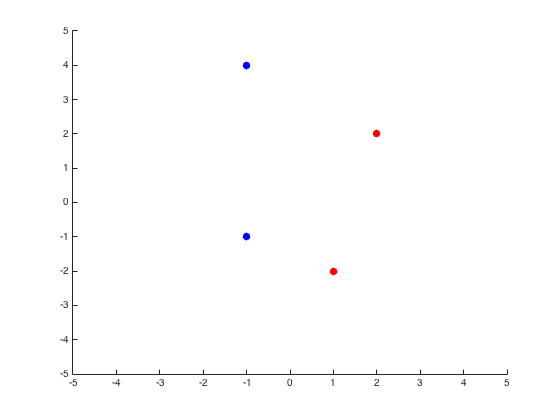
\includegraphics[width=\textwidth]{ClassifierToy_scatter.png}
\end{figure}
\end{frame}

%%%%%%%%%%%%%%%%%%
\begin{frame}{Linear Classifier: Toy Example}
Initialize: $x^{(0)} = [\frac{1}{2}, \frac{1}{2}]$.
\begin{figure}
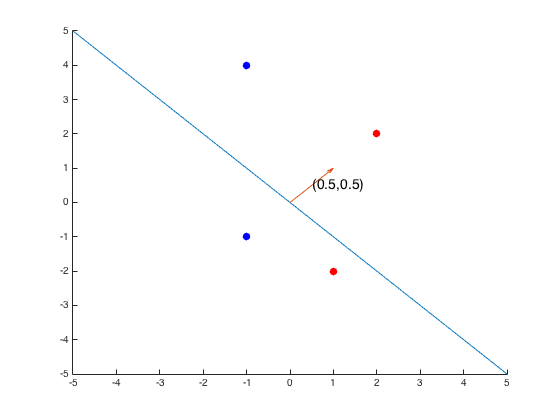
\includegraphics[width=\textwidth]{ClassifierToy_x0.png}
\end{figure}
\end{frame}

%%%%%%%%%%%%%%%%%%
\begin{frame}{Linear Classifier: Toy Example}
Misclassified example yields gain of $m^{(0)} = [\frac{1}{2},-1]$.
\begin{figure}
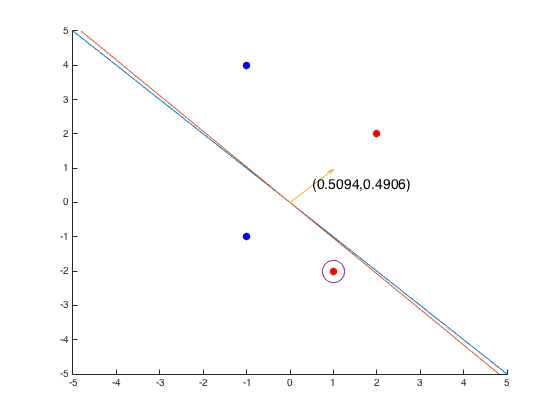
\includegraphics[width=\textwidth]{ClassifierToy_x1.png}
\end{figure}
\end{frame}

%%%%%%%%%%%%%%%%%%
\begin{frame}{Linear Classifier: Toy Example}
Continued iterations:
\begin{figure}
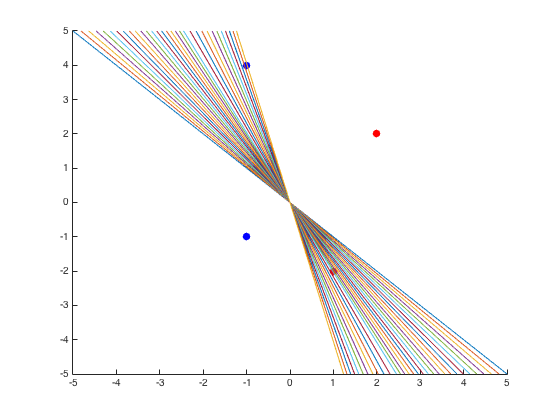
\includegraphics[width=\textwidth]{ClassifierToy_xAll.png}
\end{figure}
\end{frame}

%%%%%%%%%%%%%%%%%%
\begin{frame}{Linear Classifier: Toy Example}
Final separating hyperplane, and solution to the LP:
\begin{figure}
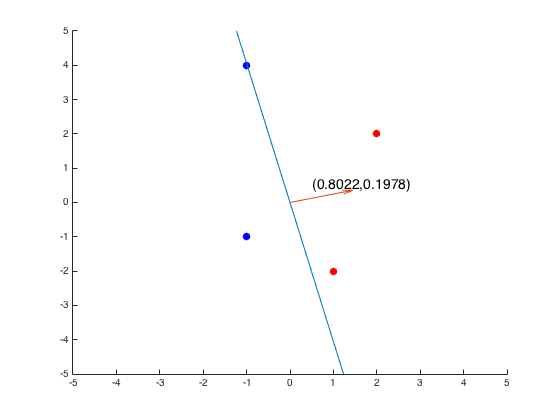
\includegraphics[width=\textwidth]{ClassifierToy_xEnd.png}
\end{figure}
\end{frame}

%%%%%%%%%%%%%%%%%%
\begin{frame}{Larger linear classifier problem}
500 labeled examples
% 65 iterations
\begin{figure}
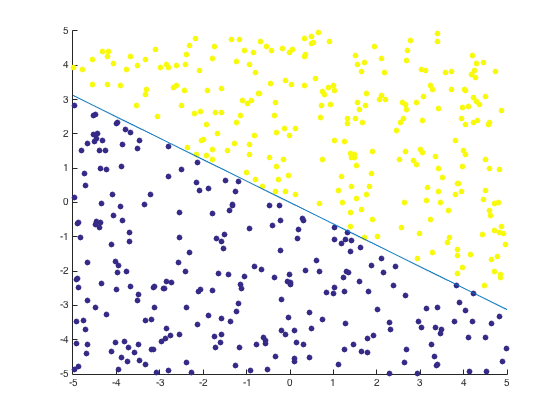
\includegraphics[width=\textwidth]{Classifier500.png}
\end{figure}
\end{frame}

%%%%%%%%%%%%%%%%%
\section[MW for SDP]{MW Algorithm for Semidefinite Programming}
\begin{frame}{Outline}
  \tableofcontents[currentsection]
\end{frame}

%%%%%%%%%%%%%%%%
%\begin{frame}{}
%\begin{itemize}
%\item Decisions are unit vectors $v$ on the unit sphere
%\item Density matrix $P^{(t)} \in \mathbb{R}^{n \times n}$, with $P \succcurlyeq 0$ and $\text{tr}(P) = 1$ \\
%Eigendecomposition of $P$: \\
%$$P = \sum_{i=1}^n \lambda_i v_iv_i^T$$
%$\lambda_i$ is the probability of $v_i$
%\end{itemize}
%\end{frame}

%%%%%%%%%%%%%%%%%
\begin{frame}{Matrix MW Algorithm}
Solving an SDP using Multiplicative Weights algorithm: \\ \vspace{.5cm}
\begin{columns}[T]
\column{.4\textwidth}
Recall the LP: 
\begin{align*}
a_j^Tx &\geq 0 \quad \forall j \\
\mathds{1}^Tx &= 1 \\
x_i &\geq 0 \quad \forall i
\end{align*}
\column{.5\textwidth}
Now the SDP:
\begin{align*}
A_j \bullet X &\geq 0 \quad \forall j = 1,\ldots,m \\
\text{Tr}(X) &= 1 \\
X & \in \mathbb S_+^n
\end{align*}
\end{columns}
\end{frame}

%%%%%%%%%%%%%%%%%%
%\begin{frame}{Bounds on the Optimal Value}
%$$\lambda_{min} \leq opt value \leq (value from thm)$$
%\end{frame}

%%%%%%%%%%%%%%%%%%
\begin{frame}{Matrix MW Algorithm}
Define $\rho = \max_j ||A_j||$, $\eta = -\text{ln}(1-\epsilon), \epsilon > 0$. \\ \vspace{.5cm}
Initialize $W^{(0)} = I_n$ \quad and $X^{(0)} = W^{(0)}/Tr(W^{(0)})$ . \\ \vspace{.5cm}
While $\exists \; j$ s.t. $A_j \bullet X^{(t)} < 0$:
\begin{enumerate}
\setlength\itemsep{1.2em}
\item Find the index $j$ such that $A_j \bullet X^{(t)} < 0$
\item Obtain the payoff $M^{(t)} = \frac{A_j}{\rho}$
\item Update the weight matrix $W^{(t)}$ and $X^{(t)}$:
$$ W^{(t+1)} = \exp \left(\eta \sum_{\tau =1}^t M^{(\tau)}\right)$$
$$
X^{(t+1)} = \frac{W^{(t+1)}}{Tr(W^{(t+1)})}
$$
\end{enumerate}
\end{frame}

%%%%%%%%%%%%%%%%%%
\begin{frame}{Recall the MAXCUT problem}
Given a weighted graph $G = (E, V)$, find a partition of the vertices into two vertex sets $V_1$ and $V_2$, i.e., $V = V_1\bigcupdot V_2$, that maximizes the ``cut'' edge weights.\\
\vspace{2cm}
(pic of graph)
\end{frame}

%%%%%%%%%%%%%%%%%%%
\begin{frame}{Recall the MAXCUT problem}
For a graph $G = (E,V)$ with $|V| = n$ and $V = V_1 \bigcupdot V_2$, the vector $x \in \mathbb{R}^n$ gives the partition:
$$
x_i = \begin{cases} 1, & \text{if } v_i \in V_1 \\
-1 , & \text{if } v_i \in V_2
\end{cases} \quad i = 1, \dots, n
$$
Let $w_{ij} := $ the weight on edge $(i,j)$
$$
\max_{x \in \{-1,1\}^n}\;\;  \sum_{(i,j) \in E} w_{ij}\frac{1-x_ix_j}{2}
$$
\end{frame}

%%%%%%%%%%%%%%%%%%%
\begin{frame}{The MAXCUT relaxation}
Introduce the auxiliary matrix variable $X = xx^T$:
\begin{align*}
\max_{x,X} \;\;  & \sum_{(i,j) \in E} w_{ij}\frac{1-x_ix_j}{2} \\
\text{s.t.} \;\; & X = xx^T \\
 & x_i^2 = 1
\end{align*}
Then drop the rank 1 constraint for the relaxation:

\begin{minipage}{0.6\linewidth}


\begin{align*}
\max_{X} \;\;  & \frac{1}{4} L \bullet X \\
\text{s.t.} \;\; & X_{ii} = 1 \quad \forall \; i=1\,\ldots,n\\
 & X \succcurlyeq 0
\end{align*}

\end{minipage}
\begin{minipage}{0.3\linewidth}

$$
L_{ij} = \left\{ \begin{aligned}
\sum _{k\in V} w_{ik},  \quad & i = j \\
-w_{ij}, \quad & i \neq j
\end{aligned}\right.
$$

\end{minipage}
\end{frame}

%%%%%%%%%%%%%%%%%%
\begin{frame}{Reformulating the MAXCUT relaxation}
Decision form: Does there exist a $b$ such that
\begin{align*}
\frac{1}{4} L \bullet X &\geq b \\
X_{ii} &= 1 \quad \forall \; i=1\,\ldots,n\\
X &\succcurlyeq 0
\end{align*}
Observe that $X_{ii} = 1 \implies (e_ie_i^T)\bullet X = 1$. Rescale $X$ by $\frac{1}{n}$. Arrive at the formulation:
\begin{align*}
\left(\frac{n}{4b} L - I\right) \bullet X &\geq 0 \\
\left(n(e_ie_i^T) - I\right) \bullet X &\geq 0 \quad \forall \; i = 1,\ldots,n \\
\text{Tr}(X) &= 1 \\
X &\succcurlyeq 0
\end{align*}
\end{frame}

%%%%%%%%%%%%%%%%%%%%

\begin{frame}{Reformulating the MAXCUT relaxation}
Let $A_j = n(e_je_j^T) - I$, $j = 1, \dots, n$ and $A_{n+1} = \frac{n}{4b} L - I$. 

\begin{align*}
A_j \bullet X &\geq 0 \quad \forall \; j = 1,\ldots,n \\
A_{n+1} \bullet X &\geq 0 \\
\text{Tr}(X) &= 1 \\
X &\succcurlyeq 0
\end{align*}
\end{frame}


\begin{frame}{Matrix MW algorithm for MAXCUT (Large-Margin)}
Define $\rho = \max_j ||A_j||$, $\eta = -\text{ln}(1-\epsilon), \epsilon > 0$, $\delta > 0$. \\ \vspace{.5cm}
Initialize $W^{(0)} = I_n$ \quad and $X^{(0)} = W^{(0)}/Tr(W^{(0)})$. \\ \vspace{.5cm}
While $\exists \; j$ s.t. $A_j \bullet X^{(t)} < -\delta$:
\begin{enumerate}
\setlength\itemsep{1.2em}
\item Find the index $j$ such that $A_j \bullet X^{(t)} < -\delta$
\item Obtain the payoff $M^{(t)} = \frac{A_j}{\rho}$
\item Update the weight matrix $W^{(t)}$ and $X^{(t)}$:
$$ W^{(t+1)} = \exp \left(\eta \sum_{\tau =1}^t M^{(\tau)}\right) ,\ \ X^{(t+1)} = \frac{W^{(t+1)}}{Tr(W^{(t+1)})}$$

\end{enumerate}
\end{frame}


%%%%%%%%%%%%%%%%%%
\begin{frame}{Toy MAXCUT problem}

Number of nodes: 4. $b^* = 16$.

\begin{table}[htbp]\label{toytable}
\centering\small
\begin{tabular}{||c|c|c|c|c||}
\hline
$\epsilon, \delta$ & 0.1 & 0.01 & 0.001 & 0.0001 \\
%\hline
%$\eta$ & 0.1054 & 0.0101 & 0.0010 & 0.0001 \\
%\hline
%$\delta$ & 0.1 & 0.01 & 0.001 & 0.0001 \\
\hline
$T$ & 20 & 328 & 3465  & 34827 \\
%\hline
%$\text{Rank} (X)$ & 4 & 4 & 4 & 4 \\
%\hline
%$\|X - X^*\|_2$ & 2.7700 & 2.7557 & 2.7556 & 2.7545 \\
%\hline
%$\|X - X^*\|_2 / \|X^*\|_2$ & 0.6925   & 0.6889 & 0.6887 & 0.6886\\
\hline
$|b^* - b|$ & 0.4595 & 0.0482 & 0.0039 & 0.0002 \\
\hline
$\frac{|b^* - b|}{|b^*|}$ & $2.88\times 10^{-2}$ &  $3.01\times 10^{-3}$  & $2.44\times 10^{-4}$ &  $1.25\times 10^{-5}$\\
\hline
\end{tabular}
\caption{toy example}
\end{table}


\end{frame}

%%%%%%%%%%%%%%%%%%
\begin{frame}{MAXCUT problem with 10 vertices}
Number of nodes: 10. $b^* = 80$. 
\begin{table}[htbp]\label{10nodestable}
\centering\small

\begin{tabular}{||c|c|c|c|c||}
\hline
$\epsilon, \delta$ & 0.1 & 0.01 & 0.001 & 0.0001 \\
%\hline
%$\eta$ & 0.1054 & 0.0101 & 0.0010 & 0.0001 \\
%\hline
%$\delta$ & 0.1 & 0.01 & 0.001 & 0.0001 \\
\hline
$T$ & 19 & 633 & 7230 & 73228 \\
%\hline
%$\text{Rank} (X)$ & 10 & 10 & 10 & 10 \\
%\hline
%$\|X - X^*\|_2$ & 8.9298 & 8.9171 & 8.9169 & 8.9168 \\
%\hline
%$\|X - X^*\|_2 / \|X^*\|_2$ & 0.8930 & 0.8917 & 0.8917 & 0.8917 \\
\hline
$|b^* - b|$ & 1.9107 & 0.1908 & 0.0204 & 0.0011 \\
\hline
$\frac{|b^* - b|}{|b^*|}$ & $2.39\times 10^{-2}$ &  $2.39\times 10^{-3}$  & $2.55\times 10^{-4}$ &  $1.38\times 10^{-5}$\\
\hline
\end{tabular}
\caption{10 nodes example}
\end{table}
\end{frame}

%%%%%%%%%%%%%%%%%%
\begin{frame}{MAXCUT problem with 100 vertices}
Number of nodes: 100. $b^* = 8190$. 
\begin{table}[htbp]\label{100nodestable}
\centering
\begin{tabular}{||c|c|c|c|c||}
\hline
$\epsilon, \delta$ & 0.1 & 0.01 & 0.001 & 0.0001 \\
%\hline
%$\eta$ & 0.1054 & 0.0101 & 0.0010 & 0.0001 \\
%\hline
%$\delta$ & 0.1 & 0.01 & 0.001 & 0.0001 \\
\hline
$T$ & 2777 & 49971 &  & \\
\hline
$|b^* - b|$ & 3.2430 & 0.7318 &  & \\
\hline
$\frac{|b^* - b|}{|b^*|}$ & $3.96\times 10^{-4}$  & $8.94\times 10^{-5}$ & & \\
\hline
\end{tabular}
\caption{100 nodes example}
\end{table}

\end{frame}

%%%%%%%%%%%%%%%%%%
\begin{frame}{Conclusions}
\begin{itemize}
\item The MW algorithm can be used to solve LP and SDP feasibility problems of certain form.
\item 
Use the MW algorithm to solve Linear Classification problems.
\item
Matrix MW algorithm performance depends on $\epsilon$ and $\delta$. (Parameter sensitive).
\end{itemize}
\end{frame}

%%%%%%%%%%%%%%%%%%
\begin{frame}{References}
\noindent
\hangindent=.7cm 
\hangafter=1
S. Arora, E. Hazan, and S. Kale. The multiplicative weights update method: A meta-algorithm and applications, \emph{Theory of Computing}, 8 (2012), pp 121-164.

\vspace{.5cm}
\noindent
\hangindent=.7cm 
\hangafter=1
S. Arora and S. Kale. A combinatorial, primal-dual approach to semidefinite programs. In \emph{Journal of the ACM}, 63 (2016).

\vspace{.5cm}
\noindent
\hangindent=.7cm 
\hangafter=1

\end{frame}


\end{document}